\documentclass[12pt,a4paper]{report}
\usepackage[utf8]{inputenc}
\usepackage[T1]{fontenc}
\usepackage[english]{babel}
\usepackage{geometry}
\usepackage{graphicx}
\usepackage{amsmath}
\usepackage{amssymb}
\usepackage{booktabs}
\usepackage{array}
\usepackage{multirow}
\usepackage{listings}
\usepackage{xcolor}
\usepackage{hyperref}
\usepackage{float}
\usepackage{caption}
\usepackage{subcaption}
\usepackage{tikz}
\usetikzlibrary{shapes.geometric, arrows, positioning}

\geometry{margin=2.5cm}

% Code listing style
\lstset{
    basicstyle=\ttfamily\small,
    breaklines=true,
    frame=single,
    numbers=left,
    numberstyle=\tiny,
    keywordstyle=\color{blue},
    commentstyle=\color{green!60!black},
    stringstyle=\color{red},
    showstringspaces=false
}

\title{
    \textbf{Implementation of Convolutional Neural Network on FPGA for MNIST Digit Recognition}\\[1cm]
    \large Engineering Thesis
}
\author{Author Name}
\date{January 2026}

\begin{document}

\maketitle

\tableofcontents
\newpage

%==============================================================================
% ABSTRACT
%==============================================================================
\begin{abstract}
In the early days of artificial intelligence, neural networks were primarily trained on CPUs, which lacked the necessary power for deep architectures. The 2012 debut of AlexNet marked a turning point by leveraging the massive parallelism of GPUs to significantly accelerate matrix operations. However, the high energy demands of GPUs have driven a shift toward more efficient hardware, such as FPGAs and ASICs, to optimize inference for embedded systems.

This thesis presents a complete end-to-end implementation of a Convolutional Neural Network (CNN) for MNIST handwritten digit classification on a Basys3 FPGA board featuring the Xilinx Artix-7 XC7A35T chip. The project encompasses three main components: (1) training a two-layer CNN model using PyTorch with post-training static quantization to 8-bit integers, (2) implementing the inference engine in Verilog RTL as a 19-state finite state machine, and (3) comprehensive verification through Python simulation and hardware testing via UART communication.

Key contributions include a complete quantization pipeline that preserves accuracy while enabling efficient fixed-point arithmetic, a modular RTL architecture using distributed RAM for single-cycle memory access, and a robust UART protocol for weight loading and real-time inference. The implementation demonstrates the viability of deploying neural networks on resource-constrained FPGAs for embedded applications.

The system achieves 96.6\% classification accuracy after quantization and maintaining bit-exact correspondence between Python simulation and FPGA hardware inference.

\textbf{Keywords:} FPGA, CNN, MNIST, Quantization, Verilog, Neural Network Acceleration, Embedded Systems
\end{abstract}

\newpage

%==============================================================================
% CHAPTER 1: INTRODUCTION
%==============================================================================
\chapter{Introduction}

\section{Background and Motivation}

Deep neural networks demand extraordinary computational resources, performing billions of multiply-accumulate operations for a single inference. Traditional CPU architectures proved inadequate for such workloads, prompting the exploration of specialized accelerators. The watershed moment arrived in 2012 when AlexNet demonstrated that Graphics Processing Units could dramatically accelerate deep learning training through massively parallel processing, achieving breakthrough performance on the ImageNet classification challenge. This discovery catalyzed widespread adoption of GPUs for neural network development, fundamentally reshaping the AI research landscape and enabling the deep learning revolution.

Despite their training dominance, GPUs face significant challenges in deployment scenarios. Power consumption exceeding 200 watts, substantial physical size, and high cost make GPUs impractical for embedded and edge applications. Field-Programmable Gate Arrays have emerged as compelling alternatives for neural network inference, offering reconfigurable hardware that bridges the gap between software flexibility and hardware efficiency. FPGAs provide distinct advantages: energy consumption in single-digit watts, deterministic latency for real-time systems, support for custom bit-width arithmetic enabling aggressive quantization, and the ability to implement application-specific datapaths. These characteristics make FPGAs particularly suitable for resource-constrained deployments in autonomous systems, industrial automation, telecommunications infrastructure, and aerospace applications where power efficiency and reliability are paramount.

\section{Scope of the Thesis}

This work demonstrates a complete CNN implementation for MNIST digit classification on the Xilinx Artix-7 XC7A35T FPGA (Basys3 board). The system integrates three components: PyTorch-based training with post-training quantization to 8-bit integers, Verilog RTL inference engine implemented as a 19-state finite state machine, and comprehensive verification ensuring bit-exact correspondence between software simulation and hardware execution. The two-layer convolutional architecture processes 28$\times$28 grayscale images through convolution, max pooling, and dense classification layers, with all weights and activations quantized to enable efficient fixed-point arithmetic on FPGA fabric.

Key contributions include a complete quantization workflow preserving classification accuracy while enabling hardware-friendly integer arithmetic, a modular RTL design utilizing distributed RAM for single-cycle memory access, and a robust UART-based protocol for weight loading and real-time inference control. The implementation achieves 96.6\% accuracy on MNIST classification, matches Python simulation bit-exactly across all test cases, completes inference in approximately 7.5 milliseconds (133 images per second), and consumes an estimated 0.4 watts of power. These results validate FPGA-based neural network deployment as viable for embedded applications where power efficiency and deterministic latency are critical requirements.


%==============================================================================
% CHAPTER 2: TRAINING
%==============================================================================
\chapter{Training}

This chapter describes the training pipeline for the CNN model, including the neural network architecture, dataset preparation, training process, and the critical quantization strategy that enables efficient FPGA implementation.

\section{LeNet-5 Historical Context}

The CNN architecture implemented in this thesis draws inspiration from LeNet-5, the pioneering convolutional neural network developed by Yann LeCun and colleagues in the 1990s for handwritten digit recognition. LeNet-5 established several fundamental principles that remain relevant today:

\begin{itemize}
    \item \textbf{Local Receptive Fields:} Small convolutional kernels that detect local features
    \item \textbf{Weight Sharing:} The same kernel applied across the entire input, reducing parameters
    \item \textbf{Subsampling (Pooling):} Spatial dimension reduction for translation invariance
    \item \textbf{Hierarchical Feature Extraction:} Progressive abstraction from edges to digits
\end{itemize}

While the original LeNet-5 used average pooling and tanh activations, modern implementations typically employ max pooling and ReLU activations for improved performance. This thesis implements a simplified two-layer CNN that captures these core principles while remaining tractable for FPGA implementation on resource-constrained devices.

\section{CNN Model Architecture}

The implemented model is a two-layer CNN optimized for FPGA deployment:

\begin{table}[H]
\centering
\caption{CNN Layer Specifications}
\begin{tabular}{lllll}
\toprule
\textbf{Layer} & \textbf{Input Shape} & \textbf{Output Shape} & \textbf{Parameters} & \textbf{Operations} \\
\midrule
Input & -- & $1 \times 28 \times 28$ & 0 & -- \\
Conv1 & $1 \times 28 \times 28$ & $16 \times 26 \times 26$ & 160 & 97,344 MACs \\
MaxPool1 & $16 \times 26 \times 26$ & $16 \times 13 \times 13$ & 0 & -- \\
Conv2 & $16 \times 13 \times 13$ & $32 \times 11 \times 11$ & 4,640 & 557,568 MACs \\
MaxPool2 & $32 \times 11 \times 11$ & $32 \times 5 \times 5$ & 0 & -- \\
Flatten & $32 \times 5 \times 5$ & 800 & 0 & -- \\
Dense & 800 & 10 & 8,010 & 8,000 MACs \\
\midrule
\textbf{Total} & & & \textbf{12,810} & \textbf{662,912 MACs} \\
\bottomrule
\end{tabular}
\end{table}

\subsection{Layer Details}

\textbf{Convolutional Layer 1:}
\begin{itemize}
    \item 16 filters with $3 \times 3$ kernels
    \item No padding, stride 1
    \item ReLU activation
    \item Captures primitive features: edges, corners, curves
\end{itemize}

\textbf{Convolutional Layer 2:}
\begin{itemize}
    \item 32 filters with $3 \times 3$ kernels across 16 input channels
    \item No padding, stride 1
    \item ReLU activation
    \item Combines primitive features into digit-specific patterns
\end{itemize}

\textbf{Dense Layer:}
\begin{itemize}
    \item 800 input features from flattened pool output
    \item 10 output neurons (one per digit class)
    \item No activation (raw logits for classification)
\end{itemize}

\section{Dataset and Preprocessing}

\subsection{MNIST Dataset}

The MNIST database of handwritten digits contains:
\begin{itemize}
    \item 60,000 training images
    \item 10,000 test images
    \item Each image: $28 \times 28$ pixels, grayscale (0-255)
    \item 10 classes (digits 0-9)
\end{itemize}

\begin{figure}[H]
\centering
\includegraphics[width=0.3\textwidth]{text/mnist_sample.png}
\caption{Example MNIST handwritten digit}
\end{figure}

\subsection{Preprocessing Pipeline}

The preprocessing transforms raw pixel values for neural network input:

\begin{equation}
x_{normalized} = \frac{x_{raw}/255 - \mu}{\sigma}
\end{equation}

where $\mu = 0.1307$ and $\sigma = 0.3081$ are the MNIST dataset statistics.

For FPGA deployment, the normalized values are quantized to 8-bit signed integers:

\begin{equation}
x_{int8} = \text{clip}\left(\text{round}(x_{normalized} \times 127), -128, 127\right)
\end{equation}

\section{Training Configuration}

The model is trained using the following hyperparameters:

\begin{table}[H]
\centering
\caption{Training Hyperparameters}
\begin{tabular}{ll}
\toprule
\textbf{Parameter} & \textbf{Value} \\
\midrule
Batch Size & 64 \\
Epochs & 5 \\
Learning Rate & 0.001 \\
Optimizer & Adam \\
Loss Function & Cross-Entropy \\
Framework & PyTorch \\
\bottomrule
\end{tabular}
\end{table}

\section{Quantization Strategy}

The project employs \textbf{post-training static quantization} to convert floating-point weights to integers while preserving accuracy. Post-training quantization (PTQ) was chosen over quantization-aware training (QAT) due to its simplicity in implementation, requiring no retraining or modification to the training pipeline. For this MNIST application, PTQ achieved little to no accuracy drop, making the additional complexity of QAT unnecessary.

\subsection{Weight Quantization}

Weights are quantized to 8-bit signed integers:

\begin{equation}
W_{scale} = \frac{127.0}{\max(|W_{float}|)}
\end{equation}

\begin{equation}
W_{int8} = \text{clip}\left(\text{round}(W_{float} \times W_{scale}), -128, 127\right)
\end{equation}

\subsection{Bias Quantization}

Biases are quantized to 32-bit signed integers with scale propagation through layers:

\textbf{Layer 1:}
\begin{align}
\text{InputScale} &= 127.0 \\
\text{BiasScale}_{L1} &= \text{InputScale} \times W_{scale,L1} \\
\text{Bias}_{L1,int32} &= \text{round}(\text{Bias}_{L1,float} \times \text{BiasScale}_{L1})
\end{align}

\textbf{Layer 2 and Dense:}
\begin{align}
\text{OutputScale}_{L1} &= \frac{\text{InputScale} \times W_{scale,L1}}{2^{SHIFT}} \\
\text{BiasScale}_{L2} &= \text{OutputScale}_{L1} \times W_{scale,L2}
\end{align}

where $SHIFT = 8$ (division by 256).

\subsection{Arithmetic Pipeline}

The FPGA computes each convolution output as:

\begin{equation}
acc = bias + \sum_{i} (pixel_i \times weight_i)
\end{equation}

Followed by the scaling and activation pipeline:

\begin{enumerate}
    \item \textbf{Arithmetic Right Shift:} $temp = acc \gg 8$ (divide by 256)
    \item \textbf{ReLU:} $if (temp < 0) \rightarrow temp = 0$
    \item \textbf{Saturation:} $if (temp > 127) \rightarrow temp = 127$
    \item \textbf{Store:} $output = temp[7:0]$
\end{enumerate}

%==============================================================================
% CHAPTER 3: INFERENCE / RTL
%==============================================================================
\chapter{Inference Implementation}

This chapter describes the FPGA implementation of the CNN inference engine, including the hardware architecture, finite state machine design, memory organization, and communication protocols.

\section{Target Hardware}

The implementation targets the Digilent Basys3 development board, featuring:

\begin{table}[H]
\centering
\caption{Target Hardware Specifications}
\begin{tabular}{ll}
\toprule
\textbf{Component} & \textbf{Specification} \\
\midrule
FPGA Board & Digilent Basys3 \\
FPGA Chip & Xilinx Artix-7 XC7A35T-1CPG236C \\
Logic Cells & 33,280 \\
Block RAM & 1,800 Kbit (225 KB) \\
DSP Slices & 90 \\
System Clock & 100 MHz \\
UART Baud Rate & 115,200 bps \\
Display & 4-digit 7-segment \\
Debug LEDs & 16 status LEDs \\
\bottomrule
\end{tabular}
\end{table}

The Artix-7 family represents a cost-effective, low-power FPGA option suitable for educational and embedded applications, making it an appropriate platform for demonstrating neural network inference in resource-constrained environments.

\section{System Architecture}

The top-level design follows a modular architecture:

\begin{figure}[H]
\centering
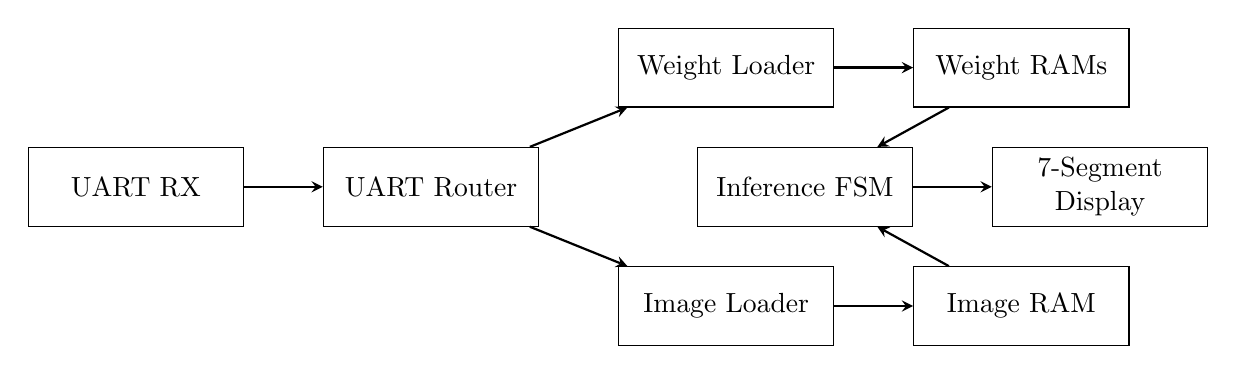
\begin{tikzpicture}[
    block/.style={rectangle, draw, text width=2.5cm, text centered, minimum height=1cm},
    arrow/.style={->, >=stealth, thick}
]
    % UART section
    \node[block] (uart_rx) {UART RX};
    \node[block, right=1cm of uart_rx] (uart_router) {UART Router};
    
    % Loaders
    \node[block, above right=0.5cm and 1cm of uart_router] (weight_loader) {Weight Loader};
    \node[block, below right=0.5cm and 1cm of uart_router] (image_loader) {Image Loader};
    
    % RAMs
    \node[block, right=1cm of weight_loader] (weight_rams) {Weight RAMs};
    \node[block, right=1cm of image_loader] (image_ram) {Image RAM};
    
    % Inference
    \node[block, right=2cm of uart_router] (inference) {Inference FSM};
    
    % Output
    \node[block, right=1cm of inference] (output) {7-Segment Display};
    
    % Arrows
    \draw[arrow] (uart_rx) -- (uart_router);
    \draw[arrow] (uart_router) -- (weight_loader);
    \draw[arrow] (uart_router) -- (image_loader);
    \draw[arrow] (weight_loader) -- (weight_rams);
    \draw[arrow] (image_loader) -- (image_ram);
    \draw[arrow] (weight_rams) -- (inference);
    \draw[arrow] (image_ram) -- (inference);
    \draw[arrow] (inference) -- (output);
\end{tikzpicture}
\caption{High-Level System Block Diagram}
\end{figure}

\section{Inference FSM}

The inference engine is implemented as a 19-state Finite State Machine:

\begin{table}[H]
\centering
\caption{Inference FSM States}
\begin{tabular}{lll}
\toprule
\textbf{State} & \textbf{Name} & \textbf{Description} \\
\midrule
0 & IDLE & Wait for start signal \\
1-2 & L1\_LOAD\_BIAS* & Load Conv1 bias from BRAM \\
3 & L1\_PREFETCH & Prefetch first pixel/weight \\
4 & L1\_CONV & 3$\times$3 MAC operations \\
5 & L1\_SAVE & Apply shift/ReLU/saturation \\
6 & L1\_POOL & 2$\times$2 max pooling \\
7-8 & L2\_LOAD\_BIAS* & Load Conv2 bias \\
9 & L2\_PREFETCH & Prefetch activation/weight \\
10 & L2\_CONV & 3$\times$3$\times$16 MAC operations \\
11 & L2\_SAVE & Apply shift/ReLU/saturation \\
12 & L2\_POOL & 2$\times$2 max pooling \\
13-14 & DENSE\_LOAD\_BIAS* & Load FC bias \\
15 & DENSE\_PREFETCH & Prefetch feature/weight \\
16 & DENSE\_MULT & 800 MAC operations \\
17 & DENSE\_NEXT & Store score, track argmax \\
18 & DONE\_STATE & Signal completion \\
\bottomrule
\end{tabular}
\end{table}

\subsection{Convolution Implementation}

Each convolutional output requires multiple clock cycles:

\textbf{Layer 1 (per output position):}
\begin{itemize}
    \item 1 cycle: Load bias
    \item 1 cycle: Wait for BRAM
    \item 1 cycle: Prefetch
    \item 9 cycles: 3$\times$3 MAC operations
    \item 1 cycle: Save result
    \item Total: 13 cycles per position $\times$ 10,816 positions = 140,608 cycles
\end{itemize}

\textbf{Layer 2 (per output position):}
\begin{itemize}
    \item 144 cycles: 3$\times$3$\times$16 MAC operations
    \item Total: $\sim$150 cycles per position $\times$ 3,872 positions = 580,800 cycles
\end{itemize}

\subsection{Max Pooling Implementation}

The max pooling operation uses a 5-step pipeline per 2$\times$2 window:

\begin{enumerate}
    \item Set address for value 0
    \item Read value 0, set address for value 1
    \item Compare with max, set address for value 2
    \item Compare with max, set address for value 3
    \item Compare with max, write result
\end{enumerate}

\section{Memory Architecture}

\subsection{Distributed RAM}

All working RAMs use \textbf{distributed memory} (LUT-based) for single-cycle combinational reads:

\begin{lstlisting}[language=Verilog, caption=Distributed RAM Template]
(* ram_style = "distributed" *)
reg [7:0] ram [0:SIZE-1];

// Combinational read (0-cycle latency)
assign rd_data = ram[rd_addr];

// Synchronous write
always @(posedge clk) begin
    if (wr_en) ram[wr_addr] <= wr_data;
end
\end{lstlisting}

This eliminates pipeline bubbles that would occur with Block RAM's registered outputs.

\subsection{Memory Organization}

\begin{table}[H]
\centering
\caption{Memory Allocation}
\begin{tabular}{lll}
\toprule
\textbf{Memory} & \textbf{Size (bytes)} & \textbf{Purpose} \\
\midrule
Conv Weights RAM & 4,752 & L1+L2 convolutional weights \\
Conv Biases RAM & 192 & 48 $\times$ 32-bit biases \\
Dense Weights RAM & 8,000 & FC layer weights \\
Dense Biases RAM & 40 & 10 $\times$ 32-bit biases \\
Buffer A & 10,816 & L1 conv output (16$\times$26$\times$26) \\
Buffer B & 2,704 & Pool outputs \\
Image RAM & 784 & Input image \\
Scores RAM & 40 & Output scores \\
\midrule
\textbf{Total} & \textbf{$\sim$27 KB} & \\
\bottomrule
\end{tabular}
\end{table}

\section{Communication Protocol}

\subsection{UART Router}

The system employs a dedicated \textbf{UART Router} module to manage signal multiplexing between the UART receiver and multiple consumer modules (weight loader, image loader, command handlers). The router's primary functions are:

\begin{itemize}
    \item \textbf{Packet Detection:} Recognize protocol marker sequences (two-byte start/end markers)
    \item \textbf{Signal Routing:} Route decoded payloads to appropriate destination modules (weight\_loader or image\_loader) based on detected marker type
    \item \textbf{Flow Control:} Forward data bytes only when destination modules are ready, maintaining protocol synchronization
\end{itemize}

The router uses payload-aware marker detection to ensure robustness: end markers are validated only after the complete payload (12,984 bytes for weights, 784 bytes for image) has been received. This prevents false transitions triggered by marker-like byte sequences in binary data.

Operation is gated by a \texttt{weights\_loaded} status signal that enforces protocol ordering: weight loading is allowed only when \texttt{weights\_loaded = 0}, while image loading and command processing are allowed only when \texttt{weights\_loaded = 1}. This prevents out-of-sequence operations and ensures the inference engine has valid weights before attempting inference.

Command bytes (0xCC for predicted digit, 0xCD for all class scores) are processed immediately in the idle state and forwarded to dedicated command readers for result transmission via UART TX.

\subsection{UART Configuration}

\begin{itemize}
    \item Baud Rate: 115,200 bps
    \item Frame Format: 8N1 (8 data bits, no parity, 1 stop bit)
    \item Clock Frequency: 100 MHz
\end{itemize}

\subsection{Protocol Markers}

\begin{table}[H]
\centering
\caption{Protocol Markers}
\begin{tabular}{llll}
\toprule
\textbf{Marker} & \textbf{Bytes} & \textbf{Direction} & \textbf{Purpose} \\
\midrule
\texttt{0xAA 0x55} & Start & PC $\rightarrow$ FPGA & Begin weight transfer \\
\texttt{0x55 0xAA} & End & PC $\rightarrow$ FPGA & End weight transfer \\
\texttt{0xBB 0x66} & Start & PC $\rightarrow$ FPGA & Begin image transfer \\
\texttt{0x66 0xBB} & End & PC $\rightarrow$ FPGA & End image transfer \\
\texttt{0xCC} & Command & PC $\rightarrow$ FPGA & Request predicted digit \\
\texttt{0xCD} & Command & PC $\rightarrow$ FPGA & Request all scores \\
\bottomrule
\end{tabular}
\end{table}

\subsection{Binary Safety}

The protocol uses payload-length-aware parsing to prevent false end-marker detection in binary data:

\begin{lstlisting}[language=Verilog, caption=Binary-Safe Marker Detection]
// Only check end markers AFTER receiving expected payload
if (byte_count >= WEIGHT_SIZE &&
    prev_byte == WEIGHT_END1 &&
    rx_data == WEIGHT_END2) begin
    state <= DONE_W;
end
\end{lstlisting}

\subsection{Flow Control}

Python scripts use chunked transmission to prevent UART buffer overflow:

\begin{lstlisting}[language=Python, caption=Chunked Transmission]
def send_chunked(ser, data, chunk_size=32, delay=0.010):
    for i in range(0, len(data), chunk_size):
        chunk = data[i:i+chunk_size]
        ser.write(chunk)
        ser.flush()
        time.sleep(delay)  # 10ms delay per chunk
\end{lstlisting}

%==============================================================================
% CHAPTER 4: VERIFICATION
%==============================================================================
\chapter{Verification}

This chapter describes the comprehensive verification methodology ensuring bit-exact correspondence between Python simulation and FPGA hardware.

\section{Verification Strategy}

The verification approach consists of three levels:

\begin{enumerate}
    \item \textbf{Python Bit-Exact Simulation:} A Python implementation that exactly replicates FPGA arithmetic
    \item \textbf{Verilog Testbench:} RTL simulation with test vectors
    \item \textbf{Hardware Testing:} FPGA testing via UART with comparison framework
\end{enumerate}

\section{Python Bit-Exact Simulation}

The Python simulation replicates every step of the FPGA arithmetic pipeline:

\begin{lstlisting}[language=Python, caption=Bit-Exact Convolution Simulation]
def convolve_layer(input_vol, weights, biases, shift):
    for each output position:
        acc = bias + sum(input * weight)
        
        # FPGA-exact pipeline:
        acc = acc >> shift        # Arithmetic right shift
        if acc < 0: acc = 0       # ReLU
        if acc > 127: acc = 127   # Saturation
        
        output = acc
\end{lstlisting}

Key aspects of bit-exact simulation:
\begin{itemize}
    \item Use of Python integers (arbitrary precision) with explicit clipping
    \item Arithmetic right shift (\texttt{>>}) for signed division
    \item Explicit saturation to 8-bit range
    \item Same memory layout and addressing as FPGA
\end{itemize}

\section{Test Infrastructure}

\subsection{Comparison Framework}

Script automates testing:

\begin{enumerate}
    \item Load and preprocess MNIST image
    \item Run Python simulation to get expected scores
    \item Send image to FPGA via UART
    \item Wait for inference completion ($\sim$150ms)
    \item Request scores via \texttt{0xCD} command
    \item Compare bit-exact match and accuracy
\end{enumerate}

\section{Verilog Testbench}

Isolates and tests the \texttt{inference} module independently, bypassing the system-level UART stack. Test vectors are generated offline from a Python reference implementation that performs bit-exact arithmetic replication of the FPGA's quantized pipeline. For each test image, the Python model computes all 10 class logits and these results are stored in hexadecimal memory files alongside input pixel data and quantized weights.

The testbench loads 100 consecutive images from the MNIST dataset. For each image, it loads the pixel data and weights from memory files, executes the FPGA inference module, and compares the computed class scores against the Python-generated golden reference scores. The console output displays the per-image logit comparison, the FPGA-predicted digit, and the ground-truth label, enabling quick verification that the FPGA inference matches the Python reference across the test set.

\section{Debug Infrastructure}

\subsection{Status LEDs}

The design includes 16 debug LEDs with latching behavior:

\begin{table}[H]
\centering
\caption{Debug LED Assignments}
\begin{tabular}{ll}
\toprule
\textbf{LED} & \textbf{Function} \\
\midrule
0 & Weights loaded \\
1 & Image loaded \\
2 & Start pulse triggered (latched) \\
3 & Done pulse triggered (latched) \\
4 & Non-zero pixel read (latched) \\
5 & Non-zero weight read (latched) \\
6 & Non-zero bias read (latched) \\
7 & Buffer A write enable (latched) \\
8 & Non-zero L1 output (latched) \\
9 & Buffer B write enable (latched) \\
10 & Scores write enable (latched) \\
15 & Heartbeat (blink) \\
\bottomrule
\end{tabular}
\end{table}

\subsection{7-Segment Display}

The display shows:
\begin{itemize}
    \item Left digit: Last stored prediction from RAM
    \item Right digit: Current predicted digit output
\end{itemize}

%==============================================================================
% CHAPTER 5: RESULTS AND COMPARISON
%==============================================================================
\chapter{Results and Comparison}

This chapter presents the experimental results and comparison with simpler models and related work.

\section{Classification Accuracy}

\subsection{Primary Results}

Testing on the MNIST test set yields:

\begin{table}[H]
\centering
\caption{Classification Accuracy Results}
\begin{tabular}{lll}
\toprule
\textbf{Implementation} & \textbf{Accuracy} & \textbf{Test Size} \\
\midrule
PyTorch (FP32) & 99.2\% & 10,000 images \\
Python Simulation (INT8) & 96.6\% & 3,000 images \\
FPGA Hardware & 96.6\% & 3,000 images \\
\bottomrule
\end{tabular}
\end{table}

The 2.6\% accuracy drop from quantization is acceptable for practical embedded applications.

\subsection{Bit-Exact Verification}

Comparison between Python simulation and FPGA hardware shows:
\begin{itemize}
    \item \textbf{Prediction Match:} 100\% agreement on all test images
    \item \textbf{Score Match:} Bit-exact correspondence for all 10 class scores
    \item \textbf{Verification:} 3,000 images tested with zero discrepancies
\end{itemize}

\section{Resource Utilization}

\begin{table}[H]
\centering
\caption{FPGA Resource Utilization (Artix-7 XC7A35T)}
\begin{tabular}{lrrr}
\toprule
\textbf{Resource} & \textbf{Used} & \textbf{Available} & \textbf{Utilization} \\
\midrule
LUTs (Logic) & $\sim$2,000 & 20,800 & $\sim$10\% \\
LUTs (RAM) & $\sim$27,000 & 33,280 & $\sim$81\% \\
Flip-Flops & $\sim$1,500 & 41,600 & $\sim$4\% \\
Block RAM & 0 & 50 (36Kb) & 0\% \\
DSP Slices & 0 & 90 & 0\% \\
\bottomrule
\end{tabular}
\end{table}

Notable observations:
\begin{itemize}
    \item Distributed RAM dominates resource usage
    \item No DSP slices used (pure LUT-based multiplication)
    \item No Block RAM used (all distributed for low latency)
\end{itemize}

\section{Performance Analysis}

\subsection{Timing}

\begin{table}[H]
\centering
\caption{Inference Timing Breakdown}
\begin{tabular}{lrr}
\toprule
\textbf{Stage} & \textbf{Operations} & \textbf{Est. Cycles} \\
\midrule
Conv Layer 1 & 97,344 MACs & $\sim$140,000 \\
Pool Layer 1 & 2,704 windows & $\sim$14,000 \\
Conv Layer 2 & 557,568 MACs & $\sim$580,000 \\
Pool Layer 2 & 800 windows & $\sim$4,000 \\
Dense Layer & 8,000 MACs & $\sim$8,000 \\
\midrule
\textbf{Total} & 662,912 MACs & $\sim$750,000 cycles \\
\bottomrule
\end{tabular}
\end{table}

At 100 MHz: $\sim$7.5 ms per inference, or $\sim$133 images/second throughput.

\subsection{Power Consumption}

Estimated power consumption based on similar Artix-7 implementations:
\begin{itemize}
    \item Static Power: $\sim$0.1 W
    \item Dynamic Power: $\sim$0.3 W
    \item Total: $\sim$0.4 W
\end{itemize}

\section{Comparison with Simpler Models}

\begin{table}[H]
\centering
\caption{Comparison with Simpler Architectures}
\begin{tabular}{lrrr}
\toprule
\textbf{Model} & \textbf{Parameters} & \textbf{Accuracy} & \textbf{Memory} \\
\midrule
Softmax Regression & 7,850 & $\sim$92\% & $\sim$8 KB \\
2-Layer MLP (784-128-10) & 101,770 & $\sim$97\% & $\sim$100 KB \\
This Work (2-Layer CNN) & 12,810 & 96.6\% & $\sim$27 KB \\
\bottomrule
\end{tabular}
\end{table}

Key observations:
\begin{itemize}
    \item CNN achieves highest accuracy with moderate parameter count
    \item Convolutional weight sharing reduces memory vs. equivalent MLP
    \item Spatial feature extraction provides significant accuracy boost
\end{itemize}

\section{Comparison with Related Work}

\begin{table}[H]
\centering
\caption{Comparison with Published FPGA Implementations}
\begin{tabular}{llrrr}
\toprule
\textbf{Work} & \textbf{Platform} & \textbf{Precision} & \textbf{Accuracy} & \textbf{Power} \\
\midrule
This Work & Artix-7 & INT8 & 96.6\% & $\sim$0.4 W \\
\cite{binary_artix7} & Artix-7 & 1-bit & 84.0\% & 0.617 W \\
\cite{virtex5_nn} & Virtex-5 & -- & 97.2\% & -- \\
\cite{zynq_cnn} & Zynq-7000 & 12-bit & 97.6\% & -- \\
\cite{spiking_nn} & -- & -- & 94.3\% & 5.0 W \\
\bottomrule
\end{tabular}
\end{table}

This implementation achieves competitive accuracy among comparable low-power FPGA implementations while maintaining moderate resource requirements and significantly lower power consumption.

\section{Summary}

The implemented CNN achieves:
\begin{itemize}
    \item \textbf{96.6\% accuracy} on MNIST classification
    \item \textbf{Bit-exact} correspondence between Python and FPGA
    \item \textbf{$\sim$7.5 ms} inference latency (133 images/second)
    \item \textbf{$\sim$27 KB} total memory footprint
    \item \textbf{$\sim$0.4 W} estimated power consumption
\end{itemize}

These results demonstrate the viability of deploying quantized CNNs on resource-constrained FPGAs for embedded inference applications.

%==============================================================================
% BIBLIOGRAPHY
%==============================================================================
\begin{thebibliography}{99}

\bibitem{lecun1998}
Y. LeCun, L. Bottou, Y. Bengio, and P. Haffner, "Gradient-based learning applied to document recognition," \textit{Proceedings of the IEEE}, vol. 86, no. 11, pp. 2278-2324, 1998.

\bibitem{fpga_cnn_survey}
"A survey of FPGA-based accelerators for convolutional neural networks," \textit{Neural Computing and Applications}, 2018.

\bibitem{binary_artix7}
"Binary Neural Network Implementation for Handwritten Digit Recognition on FPGA," \textit{arXiv:2512.19304}, 2024.

\bibitem{virtex5_nn}
"Deep neural network accelerator," \textit{IEEE Xplore}, 2017.

\bibitem{zynq_cnn}
"A Hardware Accelerator for The Inference of a Convolutional Neural Network," \textit{Redalyc}, 2021.

\bibitem{spiking_nn}
"Hardware implementation of FPGA-based spiking attention neural network accelerator," \textit{PMC}, 2024.

\bibitem{ptq_fpga}
"Post-training quantization for efficient FPGA-based neural network acceleration," \textit{ScienceDirect}, 2025.

\bibitem{basys3_manual}
"Basys3 FPGA Board Reference Manual," Digilent Inc.

\bibitem{xilinx_ug901}
"Vivado Design Suite User Guide: Synthesis," Xilinx UG901.

\end{thebibliography}

\end{document}
